\documentclass[10pt,a4paper]{article}
\usepackage{graphicx}
\usepackage{url}
\usepackage{amssymb}
\usepackage{fullpage}
\usepackage{amsmath}

\title{Senior Nanoscience 2011 Assignment 1}
\date{}
\author{D. G. Wilcox \\
		309248035}

\begin{document}

\maketitle

\section*{Question 1}

\begin{itemize}
	\item[(a)]
	\item[(b)]
	\item[(c)]
\end{itemize}

\section*{Question 2}

\begin{itemize}
	\item[(i)] The Ballot Theroem, introduced by Joseph Bertran, is the question "In an election where candiate A recieves $p$ votes and candiate B $q$ votes, with $p > q$, what is the probability that A will be strictly ahead throughout the count?"\footnote{\url{http://en.wikipedia.org/wiki/Bertand's_ballot_theorem}}. The way this explains Brownian motion is by stating that although the amount of particles (and therefore momentum) transfered to a Brownian particle by smaller particles is likely to have a net value of zero of time, for any given instant one direction (in 3D space) will be favoured over the other directions.

	The assumptions made in order for the Ballot theorem to apply are:
		\begin{itemize}
			\item[\textbullet] A candiate from the Ballot Theorem is a direction of motion in Brownian motion.
			\item[\textbullet] That the bombadment of moment from smaller particles is not always equivalent to zero.
			\item[\textbullet] That the quantities involved (ie. mass of Brownian particle, momentum of smaller particles) are such that a significant amount of motion is produced.
		\end{itemize}
	\item[(ii)] Although the question says to provide an alternative explanation to the Ballot Theroem to explain Brownian motion I will instead make the argument that the Ballot Theorem is a viable argument and that it's assumptions are valid.

	Consider the alternative to the claim of the Ballot Theorem. In this scenario we have multidutes of particles hitting the Brownian Particle over time from all directions (in approximately equal quantities). The alternative is that for any given moment the sum of the momentum of all the particles is exactly equal to zero (or close enough as to not be recognisable as the phenomenom known as Brownian motion).

	Given the sheer magnitude of the quantities of particles involved, it is obvious that there will be an inequality in the sum of the momentums. For this scenario to not produce Brownian motion we then would have to argue that these non-zero values are close enough to zero as to not be observed. This is possible.

	However, this is but one moment, in a series of possibly thousands of moments in a single second. Even if for not just any but many given moments the sum of the momentums is close enough to zero to be unobservable, there is still likely to be a small handful of moments in which the net momentum is large enough to produce significant movement of the particle. And now, because the net momentum is so regularly insignificant, the Brownian particle will retain it's momentum in the given favoured direction until another unlikely event occurs, which may add to the moment, subtract to it, or some combination in 3D space.

	So in summary, by modelling the lifetime of a Brownian particle as a series of events, in which each event there is a net momentum that is the result of all the particles bombarding it, we have come to two outcomes:
		\begin{enumerate}
			\item The net momentum for each event is enough to produce the observed Brownian motion effect.
			\item The net momentum for each event is not enough to produce the observed Brownian motion effect. That said there are many events occuring all the time, and due to the large numbers the upper end of the distribution of net momentums is significant enough to produce Brownian motion.
		\end{enumerate}

	Note that this argument successfully defends Ballot Theorem as the cause of Brownian motion only in cases with an exceedingly high rate of events.
\end{itemize}

\section*{Question 3}

\begin{enumerate}
	\item 
		\begin{itemize}
			\item[(i)] The period of a Bragg grating is given by the formula:
				\begin{equation*}
					\lambda = 2 n \Lambda
				\end{equation*}
				where $\lambda$ is the reflected wavelength (1550.5 nm), $n$ is the refractive index (1.44), and $\Lambda$ is the period of the grating. This gives us:
				\begin{align*}
					\Rightarrow \Lambda &= \frac{\lambda}{2n} \\
					 &= \frac{1550.5 \times 10^{-9}}{2 \times 1.44} \\
					\therefore \Lambda &= 4.51 \times 10^{-7} \mbox{ m} \\
				\end{align*}
			\item[(ii)] I would guess for $\Delta n$ to be around $4.5 \times 10 ^{-4}$, as that is the typical scale for the dimensions provided.
		\end{itemize}
	\item
		\begin{itemize}
			\item[(i)] Rather then interfere two beams of light to get the diffraction pattern, the use of a glass phase mask (depicted below) can mimic the same effect. This is partly due to glass' photosensitivity to certain wavelengths, and to it's refractive index.
				\begin{figure}[!h]
					\begin{center}
						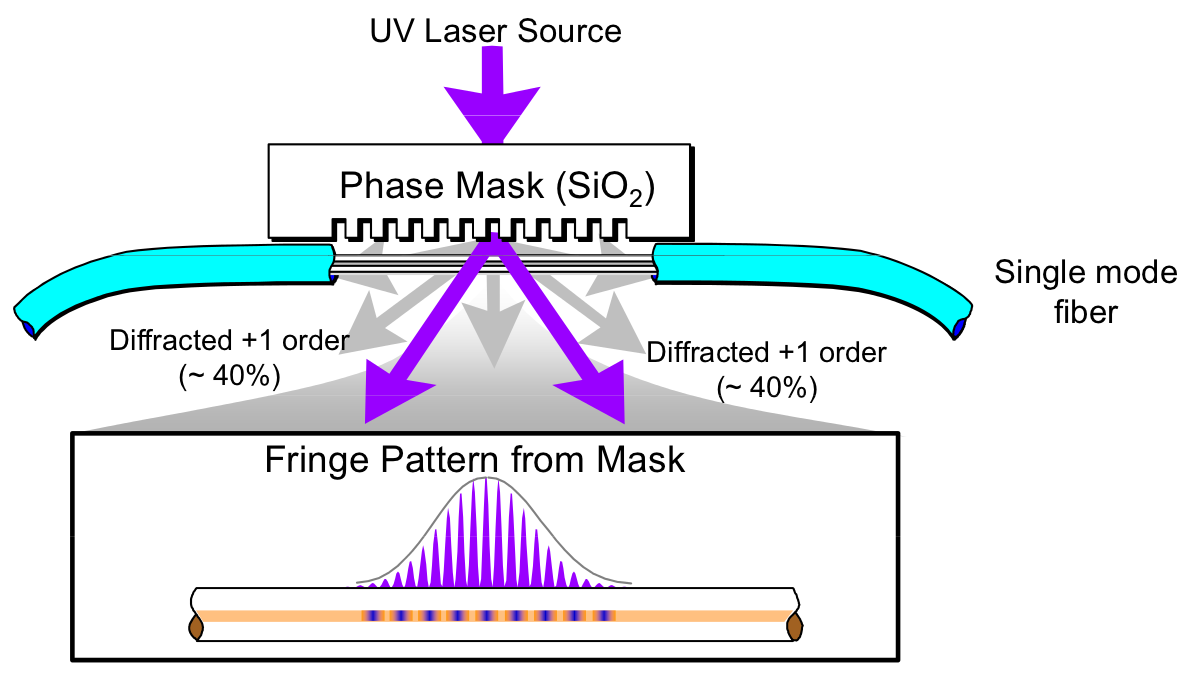
\includegraphics[width=0.7\linewidth]{phaseMask.png}
					\end{center}
					\caption{Taken from the lecture slides}
				\end{figure}
			\item[(ii)]
			\item[(iii)]
		\end{itemize}
	\item
	\item
		\begin{itemize}
			\item[(a)]
			\item[(b)]
			\item[(c)]
		\end{itemize}
\end{enumerate}

\end{document}
